% Shootout: Chapter 1 hand-typeset in memoir class, 6x9" trim.
% What raw LaTeX buys over Quarto's default book template:
%   custom chapter opener, epigraph, drop cap, margin notes, small-caps
%   lead-in, tuned float placement, custom folios/headers.
% Build: ./build.sh   (TinyTeX latexmk)
\documentclass[10pt,twoside,openright]{memoir}

% ---- trim + stock: 6x9, KDP-style margins with gutter ----
\setstocksize{9in}{6in}
\settrimmedsize{9in}{6in}{*}
\settypeblocksize{7.1in}{3.9in}{*}
\setlrmargins{0.75in}{*}{*}   % spine side wider
\setulmargins{0.7in}{*}{*}
\setmarginnotes{0.12in}{0.85in}{\onelineskip}
\checkandfixthelayout

\usepackage{lmodern}
\usepackage[T1]{fontenc}
\usepackage{microtype}
\usepackage{graphicx}
\usepackage{booktabs}
\usepackage{lettrine}
\usepackage{amsmath}

% ---- chapter opener: rules + small caps, no "Chapter N" shouting ----
\makechapterstyle{meridian}{%
  \renewcommand*{\chapterheadstart}{\vspace*{2\baselineskip}}
  \renewcommand*{\printchaptername}{}
  \renewcommand*{\printchapternum}{%
    \centering\normalfont\Large No.\;\thechapter}
  \renewcommand*{\afterchapternum}{\par\nobreak\vskip 0.5\baselineskip
    \hrule height 0.4pt \vskip 0.75\baselineskip}
  \renewcommand*{\printchaptertitle}[1]{%
    \centering\normalfont\huge\scshape ##1}
  \renewcommand*{\afterchaptertitle}{\par\nobreak
    \vskip 0.75\baselineskip \hrule height 0.4pt
    \vskip 2\baselineskip}
}
\chapterstyle{meridian}

% ---- running heads: author | title, folios in footer ----
\makepagestyle{ifm}
\makeevenhead{ifm}{}{\small\scshape rex meridian}{}
\makeoddhead{ifm}{}{\small\itshape the starlight engine}{}
\makeevenfoot{ifm}{\small\thepage}{}{}
\makeoddfoot{ifm}{}{}{\small\thepage}
\pagestyle{ifm}

\newcommand{\side}[1]{\marginpar{\footnotesize\itshape #1}}

\begin{document}

\chapter{The Giza Power Plant Problem}

\epigraph{Nobody points a 147-meter optical instrument at the brightest
available pump source by accident.}{---\textsc{r.\,meridian},
\textit{Bulletin of the IFM}, vol.~1}

\lettrine[lines=3,findent=2pt,nindent=0pt]{E}{gyptology asks} us to
believe that the Great Pyramid --- 2.3~million blocks, 5.9~million
tonnes, aligned to true north within 0.067~degrees --- is a
\emph{tomb}.\side{Petrie 1883: the survey that measured everything and
concluded furniture.} A tomb in which no mummy was ever found, built to
tolerances that modern contractors achieve only under threat of
litigation. My garage is aligned to true north within about eleven
degrees, and I have never once been buried in it.

The mainstream had their chance. Petrie surveyed the structure to two
decimal places and then, standing at the exact intersection of genius
and cowardice, concluded ``tomb.'' Dunn came closer, but thought too
small: a power plant, yes, but he never asked \emph{what the power was
for}.

\section*{The reactor hypothesis}

Consider the facts the tour guides skip. The King's Chamber is granite
--- 55~tonnes of it shipped 800~kilometers when perfectly good limestone
was lying around locally, the way you or I might import a tungsten
crucible into a house otherwise made of drywall.\side{Granite: quartz-bearing,
piezoelectric, allegedly a ceiling material.} Granite is quartz-bearing.
Quartz is piezoelectric. I trust the reader can complete the thought,
but for the slower reviewers at \textit{Nature}: \textbf{the King's
Chamber is a containment vessel}, and the sarcophagus --- granite,
lidless, acoustically resonant --- is the fusion core.

\begin{figure}[tp]
  \centering
  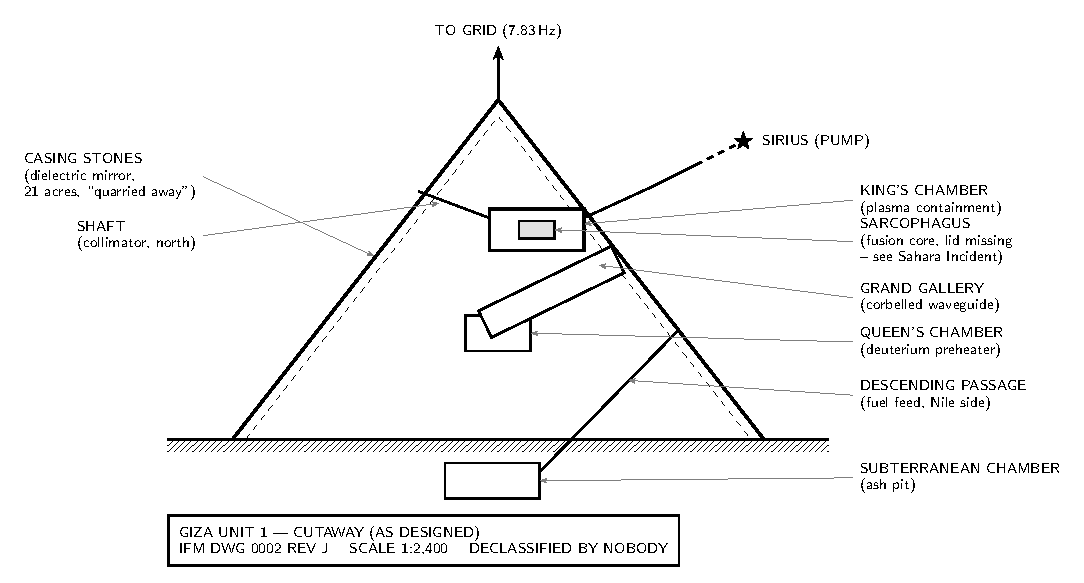
\includegraphics[width=\textwidth]{../book/figures/giza-reactor.pdf}
  \caption{Cutaway of the Giza reactor as designed. Egyptology has
  labeled every component after furniture.}
  \label{fig:reactor}
\end{figure}

\begin{table}[bp]
  \centering\small
  \begin{tabular}{ll}
    \toprule
    ``Archaeological'' name & Actual function \\
    \midrule
    King's Chamber & Plasma containment vessel \\
    Sarcophagus & Fusion core (lid ejected during excursion) \\
    Queen's Chamber & Deuterium preheater \\
    Grand Gallery & Corbelled waveguide / gain stage \\
    ``Air shafts'' & Stellar collimators (Sirius-locked) \\
    Subterranean Chamber & Ash pit \\
    Limestone casing (missing) & Dielectric mirror, 21 acres \\
    \bottomrule
  \end{tabular}
  \caption{The chamber-to-component mapping.}
  \label{tab:chambers}
\end{table}

\section*{The power budget}

The output rating falls directly out of physics that even my critics
accept. Take the pyramid's mass and the only equation the public knows:
\begin{equation}
  P_{\text{out}} \;=\; \frac{m_{\text{pyr}}\,c^{2}}{t_{\text{dynasty}}}
  \;=\; \frac{(5.9\times10^{9}\,\text{kg})\,(3\times10^{8}\,\text{m/s})^{2}}
  {\text{one dynasty}}
  \label{eq:power}
\end{equation}
The reader will object that you cannot divide by a
dynasty.\side{Working in SI dynasties. The unit is natural; the
objections are cultural.} The reader is invited to find a better unit of
time in the Egyptological literature. There isn't one. Working in SI
dynasties, equation~\eqref{eq:power} yields \textbf{1.8 × 10\textsuperscript{17}
watts of nameplate capacity} --- roughly mankind's total present
consumption, times ten thousand, which is exactly the kind of margin
you'd want if you were running a \emph{planet}.

\section*{The Sirius collimator}

The southern shaft of the King's Chamber pointed, in 2500~BC, at
Sirius. Sirius is the brightest star in our sky. The mainstream calls
this ``religious symbolism.'' I call it \textbf{aperture selection}. The
shafts are collimators; the missing casing stones --- 21~acres of
polished Tura limestone, reflectivity like a salt flat at noon --- were
the primary mirror. Starlight in, plasma confinement sustained, and the
coincidence engine warms up: the pyramid's latitude is
29.9792458°N,\side{The speed of light is 299{,}792{,}458 m/s. The same
digits. The same order. Sleep well.} and the speed of light is
299{,}792{,}458~m/s.

One question remains: 1.8 × 10\textsuperscript{17} watts is far too much
for Bronze Age toaster ovens. That surplus had a destination. Hold that
thought through the Andes.

\end{document}
